\section{Experiência de Young}
A natureza ondulatória da luz foi demonstrada no final do séc.~XVIII por um
conjunto de observações, de que se destaca uma experiência de interferência da
luz que atravessa duas fendas paralelas realizada por Young nos primeiros anos
do séc.~XIX.

Nesta experiência, faz-se incidir luz monocromática num alvo opaco com duas
aberturas com a forma de fendas finas, rectilíneas, paralelas e próximas uma da
outra, e observa-se a intensidade luminosa que é transmitida através das duas
fendas num ecrã colocado atrás do alvo (veja a Figura~\ref{fig:oof050}).
\begin{figure}[htb]
{\centering
%\includegraphics{figs/oof050.png}
\caption{Experiência de dupla fenda de Young e Fresnel.\label{fig:oof050}}

}
\end{figure}
Numa primeira abordagem, considerando apenas a lei da propagação retilínea da
luz, poderíamos pensar que o resultado desta experiência consiste na projecção
da sombra do alvo no ecrã, ficando nele definidas duas zonas iluminadas pela luz
que passa através de cada uma das fendas. No entanto, se as duas fendas
estiverem muito próximas uma da outra (a não mais do que uma ou duas décimas de
milímetro) vemos aparecer no ecrã uma série de faixas iluminadas paralelas, em
vez de duas apenas como se tenta ilustrar na Figura~\ref{fig:oof060}.
\begin{figure}[htb]
    {\centering
        %\includegraphics{figs/oof060.png}
        \caption{Padrão de interferência característico de uma experiência de
            dupla fenda.\label{fig:oof060}}

    }
\end{figure}
Este resultado pode ser compreendido à luz do princípio de Huygens. A onda
luminosa que se propaga para trás do alvo e que atinge o ecrã é a sobreposição
das duas ondas que têm origem em cada uma das fendas. Nalgumas direções, essa
sobreposição é construtiva, noutras é destrutiva e daí resulta a sucessão de
zonas iluminadas e obscuras no ecrã. Tentemos analisar isto em mais detalhe.

Seja $\lambda$ o comprimento de onda da radiação usada, $a$ a distância entre
as duas fendas e $O$ um ponto situado sobre o alvo a igual distância ($a/2$, é
claro) de ambas. Seja $F$ a localização da fonte, considerada pontual. A direção
$FO$, que une a fonte ao ponto $O$ é a direção de incidência ou direção frontal.
Seja ainda $O'$ o ponto onde esta direção interseta o ecrã (veja a
Figura~\ref{fig:oof070}).  As ondas originadas em cada fenda têm, aí, a mesma
fase (que é da onda que nelas incidiu). Mas, até atingirem o ponto $P$,
percorrem distâncias diferentes. Logo, chegam a esse ponto com fases diferentes.
Calculemos esta diferença de fases. As distâncias percorridas pelas duas ondas,
que são as distâncias que separam cada fenda do ponto $P$, são dadas por
\begin{align*}
    s_1&=\sqrt{d^2+\left(y-\frac{a}{2}\right)^2}&
    s_2&=\sqrt{d^2+\left(y+\frac{a}{2}\right)^2}
\end{align*}
onde $d$ é a distância entre o alvo e o ecrã e $y$ é a distância $O'P$,
\begin{align*}
d&=\overline{OO'}&y&=\overline{O'P}.%&s&=\overline{OP}=\sqrt{d^2+y^2}.
\end{align*}
\begin{figure}[htb]
    {\centering
        %\includegraphics{figs/oof070}
        \caption{Geometria da experiência de Young para demonstrar a
        interferência de dupla fenda.\label{fig:oof070}}

    }
\end{figure}
Como a distância entre as fendas é muito menor do que a distância alvo-ecrã,
são válidas as aproximações\footnote{Estas expressões foram obtidas usando a
fórmula de Taylor até à primeira ordem. Com uma calculadora, faça uma estimativa
do erro das aproximações para $d=1$\,m; $a=0,1$\,mm, $y=1$\,cm.}
\begin{align*}
s_1\simeq s-\frac{y}{s}\frac{a}{2}\\
s_2\simeq s+\frac{y}{s}\frac{a}{2},
\end{align*}
onde $s=\overline{OP}=\sqrt{d^2+y^2}$ representa a distância entre o ponto $O$ e
o ponto $P$.

Seja $\varphi_0$ a fase inicial (comum, já o constatámos) das duas ondas. As
fases com que atingem o ponto $P$, de acordo com a fórmula deduzida na
Secção~\ref{sec:dfidx}, são então dadas por
\begin{align*}
\varphi_1 &= \varphi_0+2\pi\frac{s_1}{\lambda}\\
\varphi_2 &= \varphi_0+2\pi\frac{s_2}{\lambda}.
\end{align*}
A diferença de fase com que atingem o ponto $P$ é, assim,
\begin{equation*}
\delta\varphi = \varphi_2-\varphi_1 =2\pi\frac{s_2-s_1}{\lambda}=
2\pi\frac{y}{s}\frac{a}{\lambda}.
\end{equation*}
Mas $y/s=\sin\theta$, de forma que se obtém, por fim,
\begin{equation*}
\delta\varphi = 2\pi\frac{a}{\lambda}\sin\theta.
\end{equation*}

Agora que temos uma expressão para a diferença de fase das duas ondas que
atingem um ponto arbitrário no ecrã, podemos usar a fórmula deduzida na
Secção~\ref{sec:sobrpos} para calcular a amplitude da onda resultante. Mas
mais interessante que o valor da amplitude é perceber em que direções é que
ocorre interferência construtiva (direções em que aquela amplitude tem um valor
elevado) ou destrutiva (aquelas onde a amplitude se anula). Para isso, chega
aplicar neste caso as condições que estabelecemos na Secção~\ref{sec:condint}.
Constatamos então o seguinte
\begin{itemize}
\item
    \textbf{Direções em que ocorre interferência construtiva}\\
    São aquelas para as quais se verifica
    \begin{align*}
    \delta\varphi &= 2\pi\frac{a}{\lambda}\sin\theta=
                    2k\pi,\quad\text{com }k=0,\pm1,\pm2,\ldots,
    \end{align*}
    ou seja, aquelas que fazem com a direção de incidência um ângulo $\theta$
    dado por
    \begin{equation*}
        \sin\theta=k\frac\lambda a,\quad k=0,\pm1,\pm2,\ldots
    \end{equation*}
\item
    \textbf{Direções em que ocorre interferência destrutiva}\\
    Nestas direções a diferença de fase deve ser um múltiplo semi-inteiro de
    $2\pi$, isto é,
    \begin{equation*}
        \delta\varphi=2\pi\frac{a}{\lambda}\sin\theta=2\left(k+\frac12\right)
        \pi,\quad k=0,\pm1,\pm2,\ldots,
    \end{equation*}
    de onde resulta
    \begin{equation*}
        \sin\theta=\left(k+\frac12\right)\frac\lambda a,\quad
        k=0,\pm1,\pm2,\ldots
    \end{equation*}
\end{itemize}

\pagebreak

\section{Interferência em reflexões múltiplas}
\begin{wrapfigure}[10]{l}{0.3\textwidth}
    {\centering
        %\includegraphics[scale=0.9]{figs/oof080}
        \caption{Interferência em reflexões múltiplas\label{fig:oof080}}

    }
\end{wrapfigure}
Considere uma película fina de um meio transparente, como a que constitui a
superfície de uma bola de sabão, a camada oleosa que frequentemente se nota nos
charcos de água em parques de estacionamento ou a cobertura anti-reflexos de
algumas lentes oftálmicas. Quando a luz incide numa destas películas, uma parte
é refletida na face onde se dá a incidência, mas outra parte é refratada para o
interior, atravessando a película até atingir a face oposta. Aí, ocorre um novo
processo de separação: uma parte é refratada para o exterior da película, a
outra é refletida de volta para a face onde se deu a incidência. Uma parte deste
raio é refratado, sobrepondo-se ao raio que se refletiu logo no momento da
primeira incidência. Como estes dois raios (o que se refletiu na face de
incidência inicial e o que se refletiu na face oposta) percorrem trajetos
diferentes e sofrem processos diferentes, apresentam, em geral, fases diferentes
quando interferem. Em que condições é essa interferência construtiva ou
destrutiva?

A resposta genérica a esta pergunta é a do costume, estabelecida na
Secção~\ref{sec:condint}: se a diferença entre as fases dos dois raios
refletidos ($r_1$ e $r_2$ na Figura~\ref{fig:oof080}) for um múltiplo inteiro de
$2\pi$, a interferência é construtiva e o reflexo, consequentemente, intenso; ao
contrário, se essa diferença de fase for um múltiplo semi-inteiro de $2\pi$, a
interferência é destrutiva, logo, o reflexo é atenuado. Devemos agora encontrar
uma expressão para a diferença de fase entre os dois raios neste problema, para
podermos concretizar esta solução. Para isso, devemos analisar os vários
processos por que passam os dois raios.

O raio que se reflete na superfície de incidência (identificado como $r_1$ na
Figura~\ref{fig:oof080}) sofre apenas o próprio processo de reflexão; o raio que
se reflete na face oposta ($r_2$), para além da reflexão, passa ainda por duas
refrações (à entrada e à saída da película) e propaga-se dentro da película
percorrendo a sua espessura nos dois sentidos. Cada um destes processos tem que
ser analisado separadamente.

\subsection*{Alterações de fase na reflexão}
As reflexões (como as refrações) são processos temporalmente descontínuos e,
por isso, é crível que possam ser acompanhadas de alterações descontínuas também
das propriedades das ondas de luz que os sofrem, incluindo da sua fase. De
facto, nas reflexões podem ocorrer (mas não ocorrem sempre) variações de fase.
Mais concretamente, verifica-se o seguinte:
\begin{itemize}
\item
    quando o índice de refração do meio onde se propaga a luz incidente é
    \emph{menor} do que o do meio contra o qual se faz a incidência, então
    \emph{ocorre uma inversão de fase}, ou seja, o raio refletido tem uma fase
    adiantada (ou atrasada, vai dar no mesmo) de $\pi$ relativamente à do raio
    incidente.
\item
    quando o meio onde se propaga a luz incidente tem índice de refração
    \emph{maior} do que o do meio contra o qual a luz incide, \emph{não há}
    qualquer variação de fase, ou seja, o raio refletido tem a mesma fase que o
    raio incidente;
\end{itemize}

Este fenómeno é semelhante à variação de fase sofrida pela reflexão de uma onda
mecânica numa corda esticada num ponto da corda onde se unem zonas de densidade
diferente. Neste caso, constata-se que se a onda se propaga numa zona da corda
de densidade mais baixa, a onda refletida tem a fase invertida relativamente à
onda incidente; mas se a onda incidente se propaga na zona da corda de densidade
mais elevada, então a onda refletida tem fase idêntica à da incidente (veja a
figura~\ref{fig:oof090}).
\begin{figure}[htb]
{\centering
%\includegraphics{figs/oof090.png}
\caption{Reflexão e refração de ondas mecânicas numa corda esticada com dois
segmentos de densidades diferentes. À esquerda, a onda incidente propaga-se no
semento menos denso e ocorre uma inversão de fase na onda refletida; à direita,
a onda incidente propaga-se no segmento mais denso e não há inversão de fase. A
onda refratada não sofre variação de fase em qualquer dos
casos.\label{fig:oof090}}

}
\end{figure}

Em resumo, a variação de fase sofrida por uma onda de luz no processo de
reflexão é dada por
\begin{equation*}
\delta\varphi_r = 
\begin{cases}
    0&\text{se } n_1>n_2\\
    \pi&\text{se } n_1<n_2,
\end{cases}
\end{equation*}
onde $n_1$ é o índice de refração do meio onde a luz incidente se propaga e
$n_2$ é o do meio contra o qual a luz incide.


\subsection*{Alterações de fase na refração}
Aqui, a situação é mais simples: nos processos de refração nunca ocorre qualquer
variação de fase da onda. Isso mesmo é de certa forma também ilustrado na
Figura~\ref{fig:oof090}, onde se pode ver que a fase da onda refratada é, nas
duas situações representadas, igual à da onda incidente.

\subsection*{Alterações de fase na propagação}
Vimos já, na Secção~\ref{sec:dfidx}, que a variação de fase de uma onda
monocromática com comprimento de onda $\lambda$ em dois pontos do seu percurso
separados por uma distância $d$ é dada por
\begin{equation*}
    \delta\varphi_p=2\pi\frac{d}{\lambda}.
\end{equation*}
Podemos pois usar esta fórmula para calcular as variações de fase sofridas pela
onda que se reflete na superfície posterior da película devidas ao trajeto de
ida e de volta até à superfície incidente. É necessário apenas notar que no
interior da película o comprimento de onda da luz tem um valor inferior ao que
apresenta no vácuo, pois a luz desloca-se no interior da película mais devagar.
Um pouco de reflexão mostra que o valor do comprimento de onda no interior da
película é $\lambda/n_p$, onde $\lambda$ representa o comprimento de onda no
vácuo e $n_p$ o índice de refração do material que constitui a película. Com
este valor alterado do comprimento de onda, a variação de fase nos dois
trajetos (de ida e no regresso) vem dada por
\begin{equation*}
\delta\varphi_p=2\times2\pi n_p\frac{s}{\lambda},
\end{equation*}
onde o factor 2 se deve ao facto de a espessura da película, $s$, ser percorrida
duas vezes (uma à ida, a outra no regresso).
\begin{center}
    \rule{2cm}{0.1mm}
\end{center}

Agora que estabelecemos expressões para o cálculo de todas as variações de fase
sofridas por cada raio, podemos calcular afase de cada um quando se recombinam
e, mais importante, podemos calcular a diferença de fase com que se sobrepõem.
Assim, podemos determinar em que condições é que essa sobreposição é construtiva
ou destrutiva.

Vejamos um exemplo. As bolas de sabão com que as crianças brincam apresentam
frequentemente reflexos coloridos e, por vezes, têm zonas que se tornam
invisíveis (normalmente no lado de cima), por não se verem nelas quaisquer
reflexos. Qual deve ser a menor espessura da película de água e sabão (com
índice de refração $n=1,33$) para a qual se anula o reflexo de um raio de luz
com comprimento de onda 520\,nm, incidindo perpendicularmente na película?

Seja $\varphi_0$ a fase do raio incidente no ponto de incidência e num dado
instante e $\varphi_1$ e $\varphi_2$ as fases dos dois raios refletidos
($\varphi_1$ a do raio que reflete na face de incidência, $\varphi_2$ a do que
se reflete na face oposta) nesse instante nos pontos em que abandonam a
película. De acordo com o referido acima sobre as variações de fase que ocorrem
nas reflexões, tendo em conta que o índice de refração da película (água com
sabão) é maior do que o do ar, concluímos que 
\begin{equation*}
\varphi_1=\varphi_0+\pi.
\end{equation*}
Já o raio que se reflete na face posta aquela onde se dá a incidência não sofre
qualquer variação de fase na reflexão, uma vez que ela se faz contra um meio
(ar) com um índice de refração inferior ao daquele onde a luz se propaga
(película). Assim, e porque não há quaisqer variações de fase nas refrações, a
fase deste raio varia apenas devido à propagação do raio no atravessar da
película nos dois sentidos. Podemos então escrever
\begin{equation*}
\varphi_2= \varphi_0+4\pi n\frac{s}{\lambda},
\end{equation*}
onde $s$ é a espessura da película e $n=1,33$ é o índice de refração da água com
sabão. A diferença de fase entre os dois raios é então
\begin{equation*}
\delta\varphi = \varphi_2-\varphi_1=4\pi n\frac{s}{\lambda}-\pi
\end{equation*}
Pretende-se determinar o menor valor de $s$ para o qual se anula o reflexo do
raio incidente, ou seja para o qual a interferência dos dois raios refletidos é
destrutiva. Mas sabemos já que esta interferência é destrutiva se
$\delta\varphi=(2k+1)\pi$, com $k=0,\pm1,\pm2,\ldots$. Então,
\begin{align*}
4\pi n\frac{s}{\lambda}-\pi&=(2k+1)\pi\\
s&=\frac{k+1}{2n}\lambda.
\end{align*}
O menor valor de $s$ (ainda positivo, é claro) obtém-se nesta fórmula tomando
$k=0$, resultando $s=\lambda/2n\simeq 195$\,nm.

\section{Difração da luz numa fenda simples}
Um dos argumentos invocados por Newton na sua oposição à teoria da natureza
ondulatória da luz foi o da propagação retilínea. Com efeito, dizia Newton, os
fenómenos ondulatórios não se propagam sempre em linha reta. Por exemplo,
podemos ouvir alguém que nos fala de detrás de uma árvore, e as ondulações da
superfície do mar ou dos lagos não ficam totalmente bloqueadas por ilhas (ver a
Figura~\ref{fig:oof100}).
\begin{figure}[htb]
    \begin{center}
        %\includegraphics{figs/oof100.jpg}
        \caption{Difração de ondas na superfície de um lago em torno de
            uma ilhota de cascalho (fonte:
            \protect\url{http://gravelbeach.blogspot.pt/2011/12/ala-spit_15.html}).
        \label{fig:oof100} }
\end{center}
\end{figure}
Estas ondas (pelo menos as de
som e as do mar), têm a capacidade de se encurvarem, rodeando parcial ou
totalmente os obstáculos que encontram no seu caminho, efeito que tem o nome de
\emph{difração}. Ora, dizia ainda Newton, nada de parecido se podia observar
para a luz, pelo que ela não podia, assim, ser considerada como um fenómeno
ondulatório. 

Mas a verdade é que a luz apresenta também fenómenos de difração, embora com
muito menor intensidade do que o som ou as ondas do mar, pelo menos em condições
habituais. Nesta secção estudaremos a difração da luz na passagem através de uma
fenda fina aberta num obstáculo opaco. O ponto de partida é o princípio de
Huyghens: cada ponto numa frente de onda é fonte de ondas esféricas que
interferem mutuamente no avanço da frente de onda. Ou seja, o valor da função de
onda em cada ponto e em cada instante é o que resulta da sobreposição das ondas
originadas nos vários pontos da frente de onda em instantes anteriores.

Consideremos então radiação que incide num obstáculo opaco, onde se abriu uma
fenda com largura $a$, centrada na origem (ver a Figura~\ref{fig:oof110}).
Pretende-se determinar a função de onda difratada numa direção que faz com
a direção de incidência (o eixo dos $x$, na figura) um ângulo $\theta$.
\begin{figure}[htb]
    \begin{center}
        \small
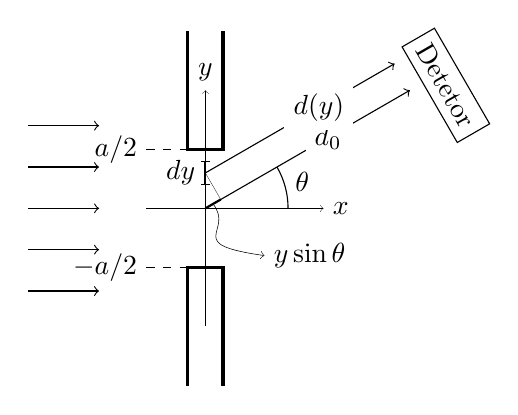
\begin{tikzpicture}[scale=1.5]
\draw [ultra thin, ->](-0.5,0)--(1,0) node [right]{$x$};
\draw [ultra thin, ->](0,-1.)--(0,1.) node [above]{$y$};
\draw [very thick](-0.15,-1.5) -- (-0.15,-0.5) -- (0.15,-0.5) -- (0.15,-1.5);
\draw [very thick](-0.15,1.5) -- (-0.15,0.5)--(0.15,0.5)--(0.15,1.5);
\draw [ultra thin, dashed] (-0.5,0.5) node [left] {$a/2$}--(-0.15,0.5);
\draw [ultra thin, dashed] (-0.5,-0.5) node [left] {$-a/2$}--(-0.15,-0.5);
\draw [->](0,0)--(30:2) node [pos=0.6,fill=white] {$d_0$};
\draw [->](0,0.3)--++(30:1.85) node[pos=0.6,fill=white] {$d(y)$};
\draw(-0.035,0.2)--(0.035,0.2);
\draw(-0.035,0.4)--(0.035,0.4);
\draw[thick](0,0.2)--(0,0.4) node[midway,left]{$dy$};
\node (D) at (1.8,1.45) [rotate=-60,right,draw] {Detetor};
\draw [ultra thin](0,0.3)--++(-60:0.26);
\draw [thick] (0,0)--(30:0.15);
\draw (0.7,0) arc (0:30:0.7);
\node at (15:0.85){$\theta$};
\draw [very thin, ->] ++(30:0.075) .. controls (0.25,-0.2) and (-0.2,-0.3) ..(0.5,-0.4) node [right]{$y\sin\theta$};
\draw [->] (-1.5, 0.70)--(-0.9,00.70);
\draw [->] (-1.5, 0.35)--(-0.9, 0.35);
\draw [->] (-1.5, 0.00)--(-0.9, 0.00);
\draw [->] (-1.5,-0.35)--(-0.9,-0.35);
\draw [->] (-1.5,-0.70)--(-0.9,-0.70);
\end{tikzpicture}
\end{center}
\caption{Difração por uma fenda simples.\label{fig:oof110}}
\end{figure}
Seja $d_0$ a distância que separa o centro da fenda do ponto onde queremos
determinar a função de onda e $d(y)$ a distância de um ponto da fenda com
ordenada $y$ até esse mesmo ponto. A contribuição que a porção infinitesimal de
fenda com comprimento $dy$ representada na figura dá para a função de onda no
ponto onde a queremos determinar é 
\begin{equation*}
    d\psi = \frac{A}{a}dy\cos\left(2\pi\left[\frac{d(y)}{\lambda}-\frac{t}{T}
    \right]\right),
\end{equation*}
onde $A$ é um fator proporcional à amplitude da onda incidente\footnote{Este
    fator depende ainda de outras variáveis, nomeadamente a distância ao
    detetor, mas que não queremos agora considerar. O que queremos, de facto,
    enfatizar, é que a amplitude da onda difratada na fenda é, em qualquer ponto
do espaço, proporcional à amplitude da onda incidente.}, e $\lambda$ e $T$ são, respetivamente,
o comprimento de onda e o período dessa onda e escolhemos nula a constante de
fase.  Mas $d(y)=d_0-y\sin\theta$. Então
\begin{equation}
    d\psi = \frac{A}{a} dy\cos\left[\Omega(t)-\strut\phi(y)\right],\label{eq:oo010}
\end{equation}
tendo-se introduzido os símbolos
\begin{align*}
    \Omega(t)&=2\pi\left(\frac{d_0}{\lambda}-\frac{t}{T}\right)&
    \phi(y)&=2\pi \frac y \lambda \sin\theta
\end{align*}
para aligeirar a notação. A função de onda resultante no ponto onde a queremos
calcular é a soma de um número infinito de contribuições semelhantes à da
eq.~\eqref{eq:oo010}, uma por cada ponto da frente de onda que atravessa a
abertura, ou seja, uma por cada ponto do eixo dos $y$ no intervalo
$[-a/2,\,a/2]$, ou seja ainda,
\begin{equation*}
    \psi=\int_{-a/2}^{a/2}\frac{A}{a}\cos\left[\strut\Omega(t)-\phi(y)\right]dy.
\end{equation*}
Usando a igualdade trigonométrica $\cos(a+b)=\cos a\cos b-\sin a\sin b$, este
integral pode escrever-se como
\begin{equation*}
    \psi=\frac{A}{a}\cos\Omega(t)\int_{-a/2}^{a/2}\cos\phi(y)\,dy+
         \frac{A}{a}\cos\Omega(t)\int_{-a/2}^{a/2}\sin\phi(y)\,dy,
\end{equation*}
uma vez que como o termo $\Omega(t)$ não depende de $y$, $\cos\Omega$ e
$\sin\Omega$ podem ser postos em evidência nos respetivos integrais. Seja agora
$\mu=2\pi/\lambda\;\sin\theta$. Então, para o primeiro destes integrais temos
\begin{align*}
    \int_{-a/2}^{a/2}\cos\phi\,dy&=\int_{-a/2}^{a/2}\cos\mu y\,dy=
    \left[\frac{1}{\mu}\sin\mu y\right]_{-a/2}^{a/2}=
    \frac2{\mu}\sin\frac{\mu a}2.
\end{align*}
Da mesma maneira, para o segundo,
\begin{align*}
    \int_{-a/2}^{a/2}\sin\phi\,dy&=\int_{-a/2}^{a/2}\sin\mu y\,dy=
    \left[\frac{1}{\mu}\cos\mu y\right]_{-a/2}^{a/2}=0.
\end{align*}
Juntando estes dois resultados, obtemos, por fim,
\begin{equation*}
    \psi = A\,\frac{\sin(\mu a/2)}{\mu a/2}\,\cos\Omega(t).
\end{equation*}
Esta equação mostra que a natureza da onda não se altera quando atravessa a
fenda, no sentido em que o seu comprimento de onda e período se mantêm (recorde
que estes parâmetros estão integrados no termo $\Omega(t)$). No entanto, a
direção de propagação deixa de ser única. Em vez disso, nota-se agora que a onda
se espalha num leque de direções, tendo uma amplitude variável dada por
\begin{equation*}
    A(\theta)=A\frac{\sin(\mu a/2)}{\mu
    a/2}=Aj_0(\pi\frac{a}{\lambda}\sin\theta),
\end{equation*}
onde se introduziu a chamada \emph{função esférica de Bessel de ordem zero}
$j_0(x)=\sin x/x$. A intensidade do sinal ondulatório, que, como vimos, é
proporcional ao quadrado da amplitude, é então
\begin{equation}
    I(\theta)= I_0 j_0^2(\pi\frac{a}{\lambda}\sin\theta),
\end{equation}
onde $I_0=I(\theta=0)$. A Figura~\ref{fig:oof120} mostra o gráfico da
intensidade da difração como função do ângulo da direção da radiação difratada,
para dois valores diferentes do quociente entre a largura da fenda e o
comprimento de onda.
\begin{figure}[htb]
\begin{center}
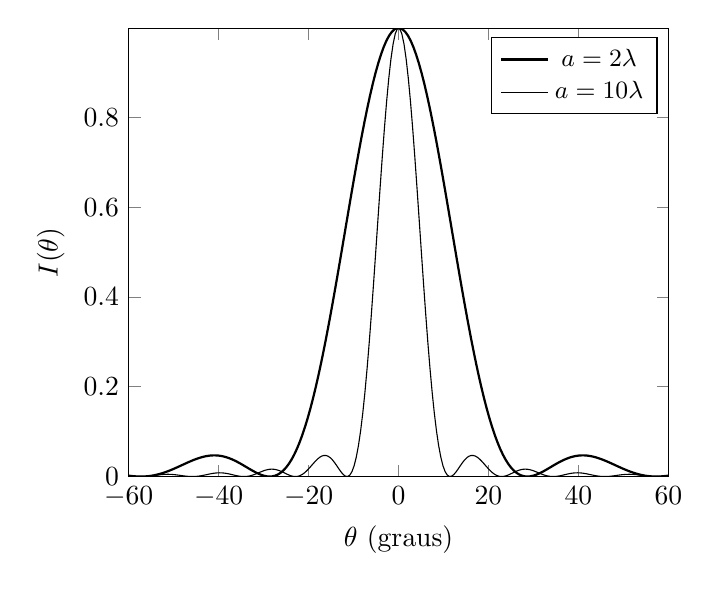
\begin{tikzpicture}
    \begin{axis}[
        enlargelimits=false,
        xlabel=$\theta$ (graus),
        ylabel=$I(\theta)$]
        \addplot [
            domain=-60:60,
            samples=200,thick
            ] {(sin(2*pi*x)/(2*pi^2*x/180))^2};
        \addlegendentry{\small $a=2\lambda$}
        \addplot [
            domain=-60:60,
            samples=250
            ] {(sin(5*pi*x)/(5*x*pi^2/180))^2};
        \addlegendentry{\small $a=10\lambda$}
    \end{axis}
\end{tikzpicture}
\caption{Intensidade da radiação difratada numa fenda simples como função do
ângulo da direção de difração (medido a partir da direção de incidência), para
$a=2\lambda$ e $a=10\lambda$.%
\label{fig:oof120}}
\end{center}
\end{figure}
Pode ver-se que a intensidade é máxima para $\theta=0$, ou seja na direção de
incidência, como seria de esperar intuitivamente, e que se reduz para zero,
tanto mais rapidamente quanto maior for a largura da abertura. A intensidade
atinge um primeiro valor mínimo mas depois apresenta oscilações com amplitude
sucessivamente menor à medida que o ângulo aumenta. Os vários mínimos de
intensidade ocorrem para ângulos $\theta_k$ dados por
\begin{equation*}
    \frac{\displaystyle%
    \sin\left(\pi\frac a \lambda \sin\theta_k\right)}{%
    \displaystyle \pi\frac a \lambda \sin\theta_k}=0.
\end{equation*}
Esta igualdade é satisfeita quando o numerador da fração se anula, sem se anular
o denominador\footnote{Se os dois --- numerador e denominador --- se anulam,
temos uma indeterminação do tipo 0/0, que, uma vez levantada, se revela
representar o valor máximo da função, em $\theta=0$!}, ou seja para
\begin{equation*}
    \pi \frac a \lambda\sin\theta_k=k\pi,\quad k=\pm1,\;\pm2,\;\pm3,\;\ldots.
\end{equation*}
O primeiro mínimo, em particular, ocorre numa direcção que faz com a de
incidência um ângulo de 
\begin{equation*}
    \theta_1 = \arcsin\frac{\lambda}{a}.
\end{equation*}
Assim, constatamos que se a largura da fenda é muito maior do que o comprimento
de onda (como certamente é o caso quando tratamos com luz e fendas ``normais,''
como janelas em paredes), então o ângulo do primeiro mínimo, que podemos tomar
como medida do espalhamento por difração, é muito pequeno, é praticamente zero.
Por isso é que não se notam, no dia a dia, efeitos da difração da luz. Mas ela
existe e pode ser demonstrada em experiências relativamente simples. Por
exemplo, a Figura~\ref{fig:oof130} mostra a sombra de uma lâmina de barbear
iluminada com raios laser. São aí claramente visíveis vários mínimos de
difração, na forma de contornos escuros em torno da sombra da lâmina.
\begin{figure}[htb]
    \begin{center}
        %\includegraphics[width=0.3\textwidth]{figs/oof130.jpg}
    \end{center}
    \caption{Difração de luz laser numa lâmina de barbear. (Fonte:
        \protect%
        \url{http://micro.magnet.fsu.edu/primer/lightandcolor/diffractionintro.html})%
    \label{fig:oof130}}
\end{figure}

\section{Polariação}
\subsection{Natureza da luz}
Os fenómenos que revelam a interferência e difração da luz mostram que a luz tem
natureza ondulatório. A luz é uma onda. Mas é uma onda de quê? Qual é a natureza
da perturbação que se propaga formando uma onda de luz? Os físicos do séc.~XIX
sopuseram que todo o universo estava preenchido com um meio material, chamado
\emph{éter lumífero,} cujas vibrações, propagando-se de ponto para ponto, seriam
a luz, como as vibrações do ar constituem o som. Como os planetas orbitam o Sol
mergulhados neste meio sem aparentemente encontrarem resistência apreciável ao
seu movimento, acreditava-se que o éter seria um fluido muito rarefeito e com
viscosidade desprezável.

Maxwell via as forças elétricas e magnéticas como resultado de tensões elásticas
deste meio. Após estabelecer as equações que foram batizadas com o seu nome,
notou que eram possíveis soluções não nulas dos campos elétrico e magnético em
regiões do espaço afastadas de fontes (cargas e correntes) desses campos. Essas
soluções eram necessariamente variáveis no tempo e os seus valores propagavam-se
de ponto para ponto com a velocidade da luz! Por isso, Maxwell propôs que a luz
era uma onda eletromagnética, o que veio a ser demonstrado em 1887 por H.~Hertz.

Assim, no final do séc.~XIX supunha-se que a luz era uma ondulação de um meio
material chamado éter lumífero, descrita matematicamente através dos campos
elétrico e magnético em conformidade com as equações de Maxwell. No entanto, não
foi possível observar o éter diretamente, ou notar efeitos inequívocos da sua
existência. Em parte por isso, Einstein propôs em 1905 que o etér não existe. A
luz (e, mais em geral, toda a radiação eletromagnética) seria apenas formada
por oscilações de uma entidade física não material, o campo eletromagnético, sem
qualquer relação com um meio corpuscular hipotético que nunca se conseguiu
observar.


\subsection{Polarização}
Uma vez que aceitamos que a radiação eletromagnética é uma oscilação do campo
eletromagnético (ou seja, do campo elétrico \emph{e} do campo magnético, que se
induzem mutuamente por indução eletromagnética), põe-se a questão de saber como
é que estes campos se comportam na presença da luz, ou, posto noutros termos,
que comportamento destes campos se traduz num fenómeno luminoso. 

De acordo com a lei de Faraday, um campo magnético variável no tempo gera uma
força eletromotriz, ou seja, um campo elétrico. Se esse campo elétrico for, por
sua vez, variável no tempo, ele gera também um campo magnético, num efeito de
indução simétrico do descrito pela lei de Faraday. Assim, perturbações
localizadas na intensidade ou na orientação de um dos (ou de ambos os) campos
podem dar origem a uma sucessão de induções de campos elétricos e magnéticos que
se propaga ao longo do espaço: assim temos uma onda de luz. 

Numa onda eletromagnética, o campo elétrico e o campo magnético são
perpendiculares entre si, e ambos perpendiculares à direção de propagação. As
orientações relativas das três direções (a de propagação, a do campo elétrico e
a do campo magnético) está ilustrada na Figura~\ref{fig:oof140}.
\begin{figure}[htb]
    {\centering

        %\includegraphics[width=0.55\linewidth]{figs/ew.pdf}

    }
    \caption{Orientações relativas da direção de propagação de uma onda
        eletromagnética (a preto) e dos campos elétrico (vermelho) e magnético
    (azul). (Adaptada de uma imagem encontrada na Wikipédia.)\label{fig:oof140}}
\end{figure}

A palavra \emph{polarização} refere-se à orientação da direção de oscilação dos
campos (e normalmente considera-se o campo elétrico) numa onda eletromagnética.
Assim, para dar um exemplo, podemos dizer que a onda representada na
Figura~\ref{fig:oof140} \emph{está polarizada} verticalmente, ou que
\emph{tem polarização} vertical, porque é essa a orientação do seu campo
elétrico.

A luz produzida pelas fontes mais comuns é o resultado da sobreposição da luz
originada de forma independente em diferentes pontos e em diferentes instantes.
Por exemplo, a luz de uma lâmpada flurescente é produzida de forma independente
em cada um dos pontos da superfície dessa lâmpada. Por isso um raio de luz
``normal'' (no sentido em que é produzido por uma destas fontes \emph{comuns}) é
a sobreposição de luz com diferentes polarizações, de luz com \emph{todas} as
polarizações possíveis. Num raio de luz normal coexistem raios de luz polarizada
em todas as direções perpendiculares à direção de propagação. Luz assim
chama-se luz \emph{não polarizada,} ou luz \emph{despolarizada.}


\subsection{Polarização da luz por filtros polarizadores}
Há materiais que absorvem com diferentes intensidades a luz que os atravessa,
conforme a sua polarização. Esta propriedade é aproveitada para a produção de
\emph{filtros polarizadores}, que absorvem completamente as componentes da luz
com polarização numa dada direção (ver a Figura~\ref{fig:oof150}), transmitindo
sem atenuação as de polarização perpendicular a essa direção. Chama-se
\emph{eixo de transmissão} do filtro à direção em que ele não absorve 
significativamente.
\begin{figure}[htb]
    {\centering

        %\includegraphics[width=0.5\linewidth]{figs/polaroidFilter.png}

    }
    \caption{Polarização da luz que atravessa um filtro polarizador. Este filtro
        absorve a raiação com polarização perpendicular às linhas nele
        desenhadas. A direção da polarização pode ser selecionada rodando o
        filtro em torno da direção de propagação. (Imagem adaptada de uma
        encontrada na Wikipedia.)\label{fig:oof150}}
\end{figure}

Consideremos um raio de luz polarizada que atravessa um filtro polarizador. Seja
$\theta$ o ângulo entre a direção de polarização da luz incidente e o eixo de
transmissão do filtro. Na passagem pelo filtro, a radiação vê anuladas as
componentes do campo perpendiculares ao eixo de transmissão. A amplitude da
oscilação do campo elétrico fica assim multiplicada por $\cos\theta$. A
intensidade da luz transmitida, sendo proporcional ao quadrado da amplitude,
fica assim dada por
\begin{equation*}
    I(\theta) = I_0\cos^2\theta.
\end{equation*}

\subsection{Polariação por reflexão}
Quando luz atravessa uma superfície de separação entre dois meios, ocorrem (já o
vimos) refração e reflexão. A forma como a intensidade do feixe incidente se
distribui pelos feixes refratado e refletido depende do ângulo de incidência e
também da polarização da luz incidente. Em geral, verifica-se que o feixe
refletido tem maior intensidade se o feixe incidente tiver polarização paralela
à superfície refletora. Assim sendo, o reflexo numa dada superfície de luz não
polarizada está parcialmente polarizado, sendo mais intensas as componentes
paralelas à superfície. A Figura~\ref{fig:oof160} tenta ilustrar este efeito.
\begin{figure}[htb]
    {\centering

        %\includegraphics[width=0.4\linewidth]{figs/polaroidReflex.png}

    }
    \caption{A luz refletida numa superfície tem maior intensidade quando a luz
        incidente tem polarização paralela à superfície. Por isso, o reflexo de
        luz não polarizada está em geral parcialmente polarizado paralelamente à
        superfície.\label{fig:oof160}}      
\end{figure}

Quando a incidência se faz numa direção particular (que depende das propriedades
dos dois meios em cuja superfície de contacto ocorre o processo) a luz refletida
fica mesmo completamente polarizada.  O ângulo de incidência nesta situação
chama-se \emph{ângulo de Brewster.}

Verifica-se que este efeito de polarização completa da luz refletida por uma
superfície ocorre quando as direções de reflexão e de refração são
perpendiculares. Consideremos luz que se propaga num meio com índice de refração
$n_1$ e que se seflete e refrata na superfície que separa esse meio de um outro
meio com índice de refração $n_2$. Suponhamos que a incidência se faz segundo o
ângulo de Brewster, $\theta_\text B$, para os dois meios, e sejam $\theta_1$ e
$\theta_2$ os ângulos de reflexão e de refração respetivamente.
De acordo com a lei de Snell, podemos escrever
\begin{minipage}[t]{0.80\linewidth}
\begin{equation*}
    n_1\sin\theta_\text B=n_2\sin\theta_2.
\end{equation*}
Por outro lado, da perpendicularidade entre as direções de reflexão e refração,
e da lei da reflexão deduzimos que
\begin{equation*}
    \theta_2=\frac{\pi}{2}-\theta_1=\frac{\pi}{2}-\theta_\text B.
\end{equation*}
\end{minipage}
\hfill
\begin{tikzpicture}[baseline={(current bounding box.north)}]
\small
\fill [gray!20] (-1,0) rectangle (1,-1);
\draw (-1,0) node[shift={(0.2,-0.2)}]{$n_2$} node[shift={(0.2,0.15)}]{$n_1$} -- +(2,0)
	;
\draw[dashed,thin] (0,-1)--+(0,1.8);
\draw [postaction={mid arrow}](-1,0.5) -- (0,0);
\draw [postaction={mid arrow}] (0,0) -- (1,0.5);
\draw [postaction={mid arrow}] (0,0) -- (0.5,-1);
\draw [thin] (0,0) +(0,0.5) arc(90:153.4:0.5) node [yshift=10]{$\theta_\text B$};
\draw [thin](0,0)+(0,0.6) arc(90:26.6:0.6) node[yshift=10] {$\theta_1$};
\draw [thin](0,0)+(0,-0.55) arc(-90:-63.4:0.55) node[yshift=-10]{$\theta_2$};
\draw [thin](0.15,0.075) -- ++(0.075,-0.15)--+(-0.15,-0.075);
\end{tikzpicture}\\[2mm]
Substituindo na igualdade acima, obtemos uma expressão para o ângulo de
Brewster:
\begin{equation*}
    \tan\theta_\text B = \frac{n_2}{n_1}.
\end{equation*}

\subsection{Atividade ótica}
\tobedone

\section{O espectro eletromagnético}
Os fenómenos óticos estudados neste capítulo, alguns deles observados no início
do séc.~XIX, demonstram a natureza ondulatória da luz. Em meados do mesmo
século, Maxwell sugeriu que a luz é uma onda eletromagnética, consistindo em
perturbações dos campos elétrico e magnético que se geram mutuamente (por
indução eletromagnética), e esta auto-geração mútua resulta na propagação das
pertubações com uma velocidade que, no vácuo, tem o valor
$c=299\,792\,458$\,m/s.

Os nossos olhos produzem sensações visuais quando são expostos a ondas
eletromagnéticas com comprimento de onda compreendido entre os 400 e os 700\,nm.
Mas há ondas eletromagnéticas com comprimentos de onda muito maiores e muito
menores do que os dessa gama. Diferentes tipos de ondas eletromagnéticas têm
nomes diferentes. Chamamos luz à radiação eletromangética a que os nossos olhos
são sensíveis, ou seja, radiação com comprimento de onda no intervalo [400\,nm,
700\,nm]\footnote{Mas frequentemente a palavra é usada
    num sentido mais alargado, como sinónimo de radiação eletromagnética em
geral.}. Com comprimentos de onda menores que a luz, falamos de raios
ultra-violeta ($\lambda\in[10\,\text{nm},400\,\text{nm}$]), raios X
($\lambda\in[1\,\text{pm},10\,\text{nm}]$) e raios gama ($\lambda<1\,$pm); com comprimentos de onda maiores
aparecem os infra-vermelhos ([700\,nm,1\,mm]), as microondas ([1\,mm, 30\,cm]) e
as ondas de rádio ($\lambda>30$\,cm). Ao conjunto de comprimentos de onda (ou de
frequências) possíveis para as ondas eletromagnéticas dá-se o nome de
\emph{espectro eletromagnético}.

